%% LyX 2.3.6.1 created this file.  For more info, see http://www.lyx.org/.
%% Do not edit unless you really know what you are doing.
\documentclass[english]{article}
\usepackage[T1]{fontenc}
\usepackage[latin9]{inputenc}
\usepackage{geometry}
\geometry{verbose,tmargin=2.5cm,bmargin=2.5cm,lmargin=2.5cm,rmargin=2.5cm}
\usepackage{graphicx}
\PassOptionsToPackage{normalem}{ulem}
\usepackage{ulem}

\makeatletter

%%%%%%%%%%%%%%%%%%%%%%%%%%%%%% LyX specific LaTeX commands.
%% Because html converters don't know tabularnewline
\providecommand{\tabularnewline}{\\}

\makeatother

\usepackage{babel}
\begin{document}
{[}SPLIT\_HERE{]}
\begin{enumerate}
\item \textbf{{[}PJC/PRELIM/9597/2015/P1/Q1{]} }

\texttt{Rainfall\_mth.csv} is a file which contains monthly total
rainfall (in millimetres), for years 1984 to 2014. The format of the
record is \textquotedblleft \textbf{\emph{{[}Year{]} M {[}Month{]}
, {[}rainfall in millimetres{]}}}\textquotedblright . Three sample
records are: 
\begin{itemize}
\item \textquotedblleft \texttt{1984M01, 251.2}\textquotedblright , which
means total rainfall for January 1984 is 251.2; 
\item \textquotedblleft \texttt{1999M07, 225.4}\textquotedblright , which
means total rainfall for July 1999 is 225.4; 
\item \textquotedblleft \texttt{2014M11, 250.8}\textquotedblright , which
means total rainfall for November 2014 is 250.8.
\end{itemize}
The total annual rainfall for a particular year can be calculated
by adding the monthly total rainfall for the twelve months. 

\subsection*{Task 1.1 }

Write program code to find total annual rainfall from 1984 to 2014
and display in a table with a heading and borders as follows: 
\noindent \begin{center}
\begin{tabular}{|c|c|}
\hline 
Year & Total Annual Rainfall (millimetres in 1 d.p.)\tabularnewline
\hline 
1984 & 2686.7\tabularnewline
\hline 
1985 & 1483.9\tabularnewline
\hline 
1986 & 2536.1\tabularnewline
\hline 
... & ... ...\tabularnewline
\hline 
... & ... ...\tabularnewline
\hline 
... & ... ...\tabularnewline
\hline 
2014 & 1538.1\tabularnewline
\hline 
\end{tabular}
\par\end{center}

\subsection*{Evidence 1: }

The program code. \hfill{}{[}7{]}

\subsection*{Evidence 2:}

Screenshot to display total annual rainfall. \hfill{}{[}1{]}

\texttt{Rainfall\_day.csv} is another file which contains number of
rainy days in a month, for years 2009 to 2014. The format of the record
is \textquotedblleft {[}Year{]} M {[}Month{]} , {[}number of days{]}\textquotedblright .
Three sample record are: 
\begin{itemize}
\item \texttt{\textquotedblleft 2009M03, 19\textquotedblright }, which means
there are 19 rainy days in March 2009;
\item \texttt{\textquotedblleft 2011M05, 15\textquotedblright }, which means
there are 15 rainy days in May 2011; 
\item \texttt{\textquotedblleft 2014M09, 9\textquotedblright }, which means
there are 9 rainy days in September 2014. 
\end{itemize}
The average rainfall for a rainy day for a particular year can be
calculated by dividing the total annual rainfall by the total number
of rainy days in a year. 

\subsection*{Task 1.2 }

Amend your program code using the following specifications: 
\begin{itemize}
\item Allow user to input a year from 2009 to 2014
\item Output error message if input is outside these years -- 2009 to 2014
\item Calculate the average rainfall for a rainy day for that year
\item Output the result 
\end{itemize}

\subsection*{Evidence 3:}

Your amended program code. \hfill{}{[}5{]}

\subsection*{Evidence 4: }

Screenshots that show 2 test cases from running Task 1.2. \hfill{}{[}2{]}

{[}SPLIT\_HERE{]}
\item \textbf{{[}PJC/PRELIM/9597/2015/P1/Q2{]} }

Quicksort is a sorting algorithm that employs a divide-and-conquer
strategy. 

Here is a high-level description of Quicksort applied to an array
A{[}0 : n -- 1{]}: 
\begin{enumerate}
\item[1.]  Select an element from A{[}0 : n -- 1{]} to be the pivot. 
\item[2.]  Rearrange the elements of A to partition A into a left subarray
and a right subarray, such that no element in the left subarray is
larger than the pivot and no element in the right subarray is smaller
than the pivot. 
\item[3.]  Recursively sort the left and the right subarrays.
\end{enumerate}

\subsection*{Task 2.1 }

Study the identifier table and incomplete quicksort algorithm. The
missing parts of the algorithm are labelled A, B and C. 
\noindent \begin{center}
\begin{tabular}{|c|c|c|}
\hline 
Variable & Data Type & Description\tabularnewline
\hline 
\hline 
ThisArray & ARRAY OF INTEGER & Array containing the dataset\tabularnewline
\hline 
First & INTEGER & First index of array\tabularnewline
\hline 
Last & INTEGER & Last index of array\tabularnewline
\hline 
Temp & INTEGER & Temporary variable\tabularnewline
\hline 
Low & INTEGER & Index of array\tabularnewline
\hline 
High & INTEGER & Index of array\tabularnewline
\hline 
Pivot & INTEGER & Reference value in array\tabularnewline
\hline 
\end{tabular}
\par\end{center}

\noindent %
\noindent\begin{minipage}[t]{1\columnwidth}%
\texttt{FUNCTION QuickSort(ThisArray, First, Last) RETURNS NULL }

\texttt{\qquad{}DECLARE Temp:INTEGER, Low:INTEGER, High:INTEGER,
Pivot:INTEGER }

\texttt{\qquad{}Low <- First }

\texttt{\qquad{}High <- Last }

\texttt{\qquad{}.........A......... //Assign reference value }

\texttt{\bigskip{}
}

\texttt{\qquad{}WHILE Low <= High }

\texttt{\qquad{}\qquad{}WHILE(ThisArray{[}Low{]} < Pivot) //Scan
left}

\texttt{\qquad{}\qquad{}\qquad{}.........B......... }

\texttt{\qquad{}\qquad{}ENDWHILE }

\texttt{\qquad{}\qquad{}WHILE(ThisArray{[}High{]} > Pivot) //Scan
right}

\texttt{\qquad{}\qquad{}\qquad{}High <- High \textendash{} 1 }

\texttt{\qquad{}\qquad{}ENDWHILE}

\texttt{\qquad{}\qquad{}IF Low <= High //Swapping }

\texttt{\qquad{}\qquad{}\qquad{}Temp <- ThisArray{[}Low{]} }

\texttt{\qquad{}\qquad{}\qquad{}ThisArray{[}Low{]} <- ThisArray{[}High{]} }

\texttt{\qquad{}\qquad{}\qquad{}ThisArray{[}High{]} <- Temp; }

\texttt{\qquad{}\qquad{}\qquad{}Low <- Low + 1 //Shift right by
1 element}

\texttt{\qquad{}\qquad{}\qquad{}High <- High - 1 //Shift left by
1 element }

\texttt{\qquad{}\qquad{}ENDIF}

\texttt{\qquad{}ENDWHILE}

\texttt{\bigskip{}
}

\texttt{\qquad{}IF First < High }

\texttt{\qquad{}\qquad{}QuickSort(ThisArray, First, High)}

\texttt{\qquad{}ENDIF}

\texttt{\qquad{}IF Low < Last}

\texttt{\qquad{}\qquad{}.........C.........}

\texttt{\qquad{}ENDIF}

\texttt{ENDFUNCTION }%
\end{minipage}

\subsection*{Evidence 5: }

What are the three missing lines of this pseudocode?\hfill{} {[}3{]}

\subsection*{Task 2.2}

Write a program to implement the quicksort. 

The program will:
\begin{itemize}
\item Call procedure \texttt{InitialiseList}. 
\item Use the function \texttt{QuickSort} to sort an array of integer \texttt{{[}435,646,344,54,23,98,789,212,847,201,733{]}}.
Copy and paste this array from the file \texttt{Number.txt} into your
program. 
\item Output the array \uline{before} and \uline{after} the quicksort
algorithm is applied.
\end{itemize}

\subsection*{Evidence 6: }

Program code for Task 2.2.\hfill{} {[}7{]}

\subsection*{Evidence 7: }

Screenshot to show running of program code in Task 2.2.\hfill{} {[}1{]}

\subsection*{Task 2.3 }

Amend the program as follows: 

The program must also output the number of function calls carried
out. 

\subsection*{Evidence 8: }

The amended program code.\hfill{} {[}3{]}

\subsection*{Task 2.4 }

By selecting different reference values (pivot) and input datasets,
and making use of the number of function calls, evaluate the efficiency
of the algorithm. 

\subsection*{Evidence 9: }

Evaluation of efficiency of quicksort algorithm with accompanying
screenshots (showing runs of function) for different reference values
and input datasets.\hfill{} {[}4{]}

{[}SPLIT\_HERE{]}
\item \textbf{{[}PJC/PRELIM/9597/2015/P1/Q3{]} }

A program is to be written to find all the words in a piece of text
and to print them in alphabetical order, together with the number
of times each word occurs. The data structure used to hold this information
will be a linked list, with each node holding a word, the number of
occurrence of that word, and a pointer to the node containing the
next word in alphabetical order. 

The program will use nodes implemented as instances of the class ListNode.
The class \texttt{ListNode} has the following properties: 
\noindent \begin{center}
\begin{tabular}{|l|l|l|}
\hline 
\multicolumn{3}{|c|}{\texttt{Class: ListNode}}\tabularnewline
\hline 
\multicolumn{3}{|c|}{Properties}\tabularnewline
\hline 
\texttt{\hspace{0.01\columnwidth}}Identifier & \texttt{\hspace{0.01\columnwidth}}Data Type & \texttt{\hspace{0.05\columnwidth}}Description\tabularnewline
\hline 
\texttt{Word} & \texttt{STRING} & The node\textquoteright s value for a word from the text \tabularnewline
\hline 
\texttt{Count} & \texttt{INTEGER} & The node's value for number of occurrences of the word\tabularnewline
\hline 
\texttt{Pointer} & \texttt{INTEGER} & The pointer for the node\tabularnewline
\hline 
\end{tabular}
\par\end{center}

A linked list is implemented as an instance of the class \texttt{LinkedList}.
The class \texttt{LinkedList} has the following properties and methods: 
\noindent \begin{center}
\begin{tabular}{|l|l|l|}
\hline 
\multicolumn{3}{|c|}{\texttt{Class: LinkedList}}\tabularnewline
\hline 
\multicolumn{3}{|c|}{Properties}\tabularnewline
\hline 
\texttt{\hspace{0.01\columnwidth}}Identifier & \texttt{\hspace{0.01\columnwidth}}Data Type & \texttt{\hspace{0.05\columnwidth}}Description\tabularnewline
\hline 
\texttt{Node} & \texttt{ARRAY{[}30{]} of ListNode} & The linked list data structure -- data values (Word \& Count) and
pointers. Array index starts at 0. For testing purposes, the dataset
has a maximum of 30 nodes. \tabularnewline
\hline 
\texttt{Start} & \texttt{INTEGER} & Index position of the node at the start of the linked list\tabularnewline
\hline 
\texttt{NextFree} & \texttt{INTEGER} & Index position of the next unused node\tabularnewline
\hline 
\end{tabular}
\par\end{center}

\noindent \begin{center}
\begin{tabular}{|l|l|l|}
\hline 
\multicolumn{3}{|c|}{\texttt{Class: LinkedList}}\tabularnewline
\hline 
\multicolumn{3}{|c|}{Methods}\tabularnewline
\hline 
\texttt{\hspace{0.01\columnwidth}}Identifier & \texttt{\hspace{0.01\columnwidth}}Data Type & \texttt{\hspace{0.05\columnwidth}}Description\tabularnewline
\hline 
Initialise & PROCEDURE & Sets all node data values to empty string (for Word) and 0 (for Count).
Set pointers to indicate all nodes are unused and linked. Initialise
values for Start and NextFree.\tabularnewline
\hline 
Update & PROCEDURE & Updates the linked list with a word read from the text\tabularnewline
\hline 
Display & PROCEDURE & Display the current state of array content and pointers in table form.\tabularnewline
\hline 
IsEmpty & FUNCTION RETURNS BOOLEAN & Test for empty linked list.\tabularnewline
\hline 
IsFull & FUNCTION RETURNS BOOLEAN & Test for no unused nodes.\tabularnewline
\hline 
\end{tabular}
\par\end{center}

The diagram shows the linked list with: 
\begin{itemize}
\item the text \textquotedblleft mary had a little lamb\textquotedblright{}
added 
\item the unused nodes linked together. 
\end{itemize}
\begin{center}
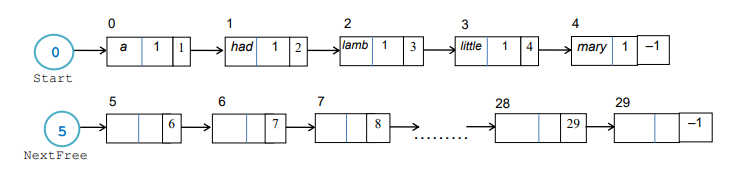
\includegraphics[width=0.65\paperwidth]{C:/Users/Admin/Desktop/Github/question_bank/LyX/static/img/9597-PJC-2015-P1-Q3-1}
\par\end{center}

\subsection*{Task 3.1}

Write the program code for the classes \texttt{ListNode} and \texttt{LinkedList},
including the \texttt{Initialise}, \texttt{Display}, \texttt{IsEmpty}
and \texttt{IsFull} method. The code should follow the specification
given. Do not write the \texttt{Update} procedure yet. 

\subsection*{Evidence 10: }

Your program code for the \texttt{ListNode} and \texttt{LinkedList}
classes. \hfill{}{[}12{]}

\subsection*{Task 3.2}

Write code to create a \texttt{LinkedList} object and run \texttt{Display}
procedure to show the content of the object. 

\subsection*{Evidence 11: }

Screenshot confirming all values after initialisation of the \texttt{LinkedList}.\hfill{}
{[}3{]}

\subsection*{Task 3.3 }

Write code to implement for the \texttt{LinkedList} class the \texttt{Update}
method that will update the linked list with a word read from the
text. 

\subsection*{Evidence 12:}

Program code for \texttt{Update} procedure. \hfill{}{[}12{]}

\subsection*{Task 3.4 }

Write code to use the Update procedure by reading in the text from
the file \texttt{Story.txt}. 

\subsection*{Evidence 13:}

Screenshot of state of array content and pointers by running \texttt{Display}
procedure. \hfill{}{[}4{]}

\subsection*{Task 3.5 }

Write a method \texttt{Query} inside \texttt{LinkedList} class that: 
\begin{itemize}
\item takes a word input by user, 
\item check if the word exists in the linked list, 
\item output appropriate message with the number of occurrences, if word
exists.
\end{itemize}

\subsection*{Evidence 14: }

Program code for \texttt{Query} method. \hfill{}{[}4{]}

\subsection*{Evidence 15: }

Screenshot from running the \texttt{Query} method for a word that
exists and another word that does not exist in the linked list. \hfill{}{[}2{]}

{[}SPLIT\_HERE{]}
\item \textbf{{[}PJC/PRELIM/9597/2015/P1/Q4{]} }

Implement a stack class using array using the following properties
and methods: 
\begin{center}
\begin{tabular}{|l|l|l|}
\hline 
\multicolumn{3}{|c|}{\texttt{Class: Stack}}\tabularnewline
\hline 
\multicolumn{3}{|c|}{Properties}\tabularnewline
\hline 
\texttt{\hspace{0.01\columnwidth}}Identifier & \texttt{\hspace{0.01\columnwidth}}Data Type & \texttt{\hspace{0.05\columnwidth}}Description\tabularnewline
\hline 
\texttt{Data} & \texttt{ARRAY{[}x{]} of STRING} & x is the limit, which must be supplied when the object is called \tabularnewline
\hline 
\texttt{Limit} & \texttt{INTEGER} & The maximum number of elements the stack can hold \tabularnewline
\hline 
\end{tabular}
\par\end{center}

\begin{center}
\begin{tabular}{|l|l|l|}
\hline 
\multicolumn{3}{|c|}{\texttt{Class: Stack}}\tabularnewline
\hline 
\multicolumn{3}{|c|}{Methods}\tabularnewline
\hline 
\texttt{\hspace{0.01\columnwidth}}Identifier & \texttt{\hspace{0.01\columnwidth}}Data Type & \texttt{\hspace{0.05\columnwidth}}Description\tabularnewline
\hline 
\texttt{IsEmpty} & \texttt{FUNCTION RETURNS BOOLEAN} & Indicates whether any elements are stored in stack or not \tabularnewline
\hline 
\texttt{IsFull} & \texttt{FUNCTION RETURNS BOOLEAN} & Indicates whether stack is full or not\tabularnewline
\hline 
\texttt{Push} & \texttt{PROCEDURE} & Inserts data onto stack\tabularnewline
\hline 
\texttt{Pop} & \texttt{PROCEDURE} & Removes and returns the last inserted element from the stack\tabularnewline
\hline 
\texttt{Peek} & \texttt{PROCEDURE} & Returns the last inserted element without removing it\tabularnewline
\hline 
\texttt{Size} & \texttt{PROCEDURE} & Returns the number of elements stored in stack \tabularnewline
\hline 
\texttt{Display} & \texttt{PROCEDURE} & Displays the content of the stack with top of stack clearly indicated\tabularnewline
\hline 
\end{tabular}
\par\end{center}

\subsection*{Task 4.1 }

Write program code for the stack class with all the properties and
methods above.

\subsection*{Evidence 16:}

Your program code. \hfill{}{[}12{]}

A stack can be used to evaluate an arithmetic expression. An arithmetic
expression can first be converted from infix notation to postfix notation,
then the postfix notation can be evaluated to get the value of the
infix notation. 

For example, the infix notation \texttt{5 {*} (6 + 2) - 12 / 4} can
first be converted to postfix notation \texttt{5 6 2 + {*} 12 4 /
-}, and then evaluated to \texttt{37} using a stack. 

The following is an algorithm for converting infix notation to postfix
notation:
\begin{enumerate}
\item[1.]  Create an empty stack called \texttt{opStack} for keeping operators. 
\item[2.]  Scan the token list from left to right. 
\begin{itemize}
\item If the token is an operand, append it to the end of the output list. 
\item If the token is a left parenthesis, push it on the \texttt{opStack}. 
\item If the token is an operator, \texttt{{*}, /, +}, or \texttt{-}, push
it on the \texttt{opStack}. However, first remove any operators already
on the \texttt{opStack} that have higher or equal precedence and append
them to the output list. 
\item If the token is a right parenthesis, pop the \texttt{opStack} until
the corresponding left parenthesis is removed. Append each operator
to the end of the output list. 
\end{itemize}
\end{enumerate}
When the input expression has been completely processed, check the
\texttt{opStack}. Any operators still on the stack can be removed
and appended to the end of the output list. 

\subsection*{Task 4.2 }

Write program code for the algorithm to convert infix notation to
postfix notation using the following specification: 
\noindent \begin{center}
\texttt{FUNCTION infixToPostfix(infixexpression:STRING):STRING}
\par\end{center}

\subsection*{Evidence 17: }

Your program code. \hfill{}{[}7{]}

The following algorithm can be used to evaluate postfix notation: 
\begin{enumerate}
\item 1. Create an empty stack called \texttt{operandStack}. 
\item 2. Scan the token list from left to right. 
\begin{itemize}
\item If the token is an operand, convert it from a string to an integer
and push the value onto the \texttt{operandStack}. 
\item If the token is an operator, \texttt{{*}, /, +, }or \texttt{-}, it
will need two operands. Pop the \texttt{operandStack} twice. The first
pop is the second operand and the second pop is the first operand.
Perform the arithmetic operation. Push the result back on the \texttt{operandStack}.
\end{itemize}
\end{enumerate}
When the input expression has been completely processed, the result
is on the stack. Pop the \texttt{operandStack} and return the value.

\subsection*{Task 4.3 }

Write program code for the algorithm to evaluate postfix notation
using the following specification: 
\noindent \begin{center}
\texttt{FUNCTION postfixEval(postfixexpression:STRING):FLOAT }
\par\end{center}

\subsection*{Evidence 18: }

Your program code.\hfill{} {[}7{]} 

\subsection*{Task 4.4}

Write program code to read the infix expressions from the file Infix.txt
and output its postfix expressions and its evaluation. 

\subsection*{Evidence 19: }

Your program code. \hfill{}{[}2{]}

\subsection*{Evidence 20: }

Screenshot of running your program code in Task 4.4.\hfill{} {[}2{]}

{[}SPLIT\_HERE{]}
\item \textbf{{[}PJC/PRELIM/9597/2015/P2/Q1{]} }

PJ Parcels is a company that specialises in the delivery and collection
of parcels for business customers. To use their services, a customer
must first register for an account. The customer needs to provide
their company name, address, telephone number and the name of a main
contact for any queries. 

As part of the registration process, the customer will have to decide
if they wish to pay monthly on receipt of an invoice, or via credit
card for each delivery made. If paying by credit card, then the card
details are also required. Once these details have been accepted,
the customer will be issued with an account number that they must
quote when contacting the company. 

When a customer requires a parcel to be delivered, they will contact
PJ Parcels to arrange collection. The customer needs to provide details
of where the parcel will be collected from; where it will be delivered
to; how many parcels are to be collected and which type of service
they want, for example, next day delivery. 

Once the collection has been arranged, an Airway Bill will be generated.
The details on this will be used by a Dispatcher to schedule the vehicle
needed for the collection. Each parcel will be given a priority number
by the Dispatcher and those with the highest priority will be collected
first. 

By 12 noon each day, the Dispatcher also needs to generate a delivery
schedule to ensure all the parcels are delivered according to the
service required.

Each Driver has a mobile device with a copy of the Airway Bill; a
person at the delivery address must sign this to say that the parcel
has been delivered. This will flag that the delivery has been completed. 

Once the parcel has been delivered, if the customer pays via credit
card, their card will be debited by the amount required, or if they
pay monthly, then the invoice account will be debited. Once a month,
the Finance Department will generate the invoices for payment. 

If the parcel cannot be delivered for any reason, it will be returned
to the Depot and a card will be left with at the delivery address
with details of how to arrange re-delivery.

The company has decided to replace this manual system with an on-line
computerised system. 

A \textbf{system developer} is employed to carry out the task. The
first task assigned to the system developer is to write a project
proposal. 
\begin{enumerate}
\item One section of the project proposal is the Problem Statement which
lists the problems in the current system. Write the Problem Statement.
\hfill{}{[}4{]}
\item The system developer (who will act as project manager) has drawn up
an initial plan of the work involved: 
\noindent \begin{center}
\begin{tabular}{|c|l|c|}
\hline 
Stage & Activity & Weeks\tabularnewline
\hline 
A & elicit requirements from the intended users, and draw up a specification & 3\tabularnewline
\hline 
B & system analysis & 2\tabularnewline
\hline 
C & system design & 7\tabularnewline
\hline 
D & system development & 5\tabularnewline
\hline 
E & system testing & 4\tabularnewline
\hline 
F & implementation of computer system & 2\tabularnewline
\hline 
G & documentation & 3\tabularnewline
\hline 
H & maintenance & 2\tabularnewline
\hline 
\end{tabular}
\par\end{center}

Task B must follow A. 

Tasks C, D and E can run concurrently, but must follow B. 

Tasks F and G can run concurrently, but cannot start until all three
tasks C, D and E have been completed. 

Task H must follow tasks F and G. 
\begin{enumerate}
\item Draw a Program Evaluation and Review Technique (PERT) chart for this
project. Use week numbers as the time units. \hfill{}{[}4{]}
\item Copy the following table and complete the earliest and latest start
and end time, and the float, for each node. 
\noindent \begin{center}
\begin{tabular}{|c|c|c|c|c|c|c|}
\hline 
Task & Duration & Earliest Start Time & Latest Start Time  & Earliest Finish Time & Latest Finish Time & Float\tabularnewline
\hline 
A & 3 & 0 & 0 & 3 & 3 & 0\tabularnewline
\hline 
B & 2 & 3 & 3 & 5 & 5 & 0\tabularnewline
\hline 
C & 7 &  &  &  &  & \tabularnewline
\hline 
D & 5 &  &  &  &  & \tabularnewline
\hline 
E & 4 &  &  &  &  & \tabularnewline
\hline 
F & 2 &  &  &  &  & 1\tabularnewline
\hline 
G & 3 & 12 &  &  & 15 & 0\tabularnewline
\hline 
H & 2 &  & 15 &  & 17 & 0\tabularnewline
\hline 
\end{tabular}
\par\end{center}
\item State the critical path. \hfill{}{[}1{]}
\item State the minimum time in which the project could be completed. \hfill{}
{[}1{]}
\item Explain dependent stages and concurrent stages. For each type of stage
give an example from this chart. \hfill{}{[}4{]}
\item Draw a Gantt chart showing all eight stages and their dependencies,
allowing for the resource allocations as indicated above. \hfill{}
{[}4{]}
\end{enumerate}
\item Identify \textbf{five} key stages with brief description of the software
development life cycle (SDLC). \hfill{}{[}5{]}
\item Explain at which stage of the SDLC was top-down analysis used, and
why it helps in the solution of complex problems. \hfill{} {[}2{]}
\item The parcel\textquoteright s data from customers entered into the new
system needs to be validated and verified. 

Explain with examples the difference between data validation and data
verification. \hfill{}{[}4{]}
\item Jane is the software testing engineer for this system. Her test strategy
includes beta testing and acceptance testing. 
\begin{enumerate}
\item Describe what is meant by beta testing and how it can be used to test
the program. \hfill{} {[}2{]}
\item Describe what is meant by acceptance testing and how it can be used
to test the program. \hfill{} {[}2{]}
\end{enumerate}
\item Some account clerks spend at least part of their week working from
home. A system analyst will assist in improving their company communication
systems. Explain why it is important to define problem accurately.
\hfill{}{[}2{]}
\item Some customers are worried because so much information is being stored
about their parcels on the server of the company. Describe the fears
that the customers may have and explain what the company can do to
allay those fears. \hfill{} {[}3{]}
\item When data is transmitted across the network it is sent in bytes. The
following bytes of data have been received by a device on the network.
\noindent \begin{center}
01101101 10110100 01101000 10100001 
\par\end{center}

One of the bytes has been corrupted.

State which is the corrupt byte, justifying your choice. \hfill{}
{[}2{]}
\item Explain how transmitting bytes in \textbf{blocks} can allow the receiving
device to selfcorrect errors. \hfill{}{[}2{]}
\item When data is transmitted on a network it can use a number of different
transmission modes. State what is meant by each of the following modes
of data transmission. 
\begin{enumerate}
\item Simplex \hfill{}{[}1{]}
\item Duplex \hfill{} {[}1{]}
\item Half-duplex \hfill{} {[}1{]}
\end{enumerate}
\end{enumerate}
{[}SPLIT\_HERE{]}
\item \textbf{{[}PJC/PRELIM/9597/2015/P2/Q2{]} }

A programmer is going to write part of the new system, using an object-oriented
programming language, which will store details of customers. All customers
will be identified by their CUST\_ID. Properties identified type of
customers is: 
\begin{itemize}
\item Payment\_type 
\end{itemize}
\begin{enumerate}
\item Draw a diagram that shows how the properties could be distributed
amongst a number of classes. Include in your diagram any inheritance
between classes. Also indicate some of the methods that would be required.
\hfill{}{[}4{]} 
\item In the context of object-oriented programming explain what is meant
by: 
\begin{enumerate}
\item encapsulation;
\item inheritance; 
\item polymorphism.\hfill{} {[}3{]}
\end{enumerate}
\item Give \textbf{two} advantages of object-oriented programming. \hfill{}{[}2{]}
\end{enumerate}
{[}SPLIT\_HERE{]}
\item \textbf{{[}PJC/PRELIM/9597/2015/P2/Q3{]} }

A recursive algorithm for finding a value, SearchItem, in an ordered
array, X, is as follows: 

\noindent %
\noindent\begin{minipage}[t]{1\columnwidth}%
\texttt{Search(Low, High) }

\texttt{\qquad{}Mid =(Low + High) div 2 }

\texttt{\qquad{}If X(Mid) = SearchItem then output \textquotedbl found\textquotedbl{}
: exit }

\texttt{\qquad{}If X(Mid) > Searchltem then Search(Low, Mid-1) }

\texttt{\qquad{}\qquad{}Else Search(Mid+1, High) }

\texttt{End Search }

\texttt{\qquad{}}Note: the \texttt{div} operation returns an integer
value after division e.g.\texttt{ 7 div 2 = 3} %
\end{minipage}

Using the above algorithm: 
\begin{enumerate}
\item Explain what is meant by a recursive algorithm. \hfill{}{[}1{]}
\item Describe what might occur during execution with an incorrectly written
recursive routine. 

Array \texttt{X} has 15 elements and the subscripts start at 1. \hfill{}
{[}2{]}
\item If the algorithm was used to search the array \texttt{X} for the value
stored at \texttt{X(3)} state the calls to Search as the recursion
executes. \hfill{} {[}2{]}
\item The algorithm does not handle the case where SearchItem is not present
in \texttt{X}. Indicate what changes need to be made to Search to
rectify this problem. \hfill{}{[}3{]}
\item For this method of searching state the maximum number of comparisons
and the minimum number of comparisons for array \texttt{X}, justifying
your answers. \hfill{}{[}2{]}
\end{enumerate}
{[}SPLIT\_HERE{]}
\item \textbf{{[}PJC/PRELIM/9597/2015/P2/Q4{]} }

An alternative solution for this project is to use cloud computing. 

Discuss briefly the \textbf{three} services that could be used for
the new project. \hfill{}{[}3{]}

{[}SPLIT\_HERE{]}
\item \textbf{{[}PJC/PRELIM/9597/2015/P2/Q5{]} }

PJC Enterprise plans to create a computer system to store data on
its employees and the insurance type and coverage for each of them.
An employee may be insured by more than one policy. A solution is
to create a database with three tables: \emph{Employee}, \emph{Insurance}
and \emph{Policy}. 

\emph{Employee} table contains information about its employees. \emph{Insurance}
table gives information on the insurance plan type and the date of
issue of the policy for an employee. \emph{Policy} table contains,
for each type of insurance plan, a description of its coverage and
its monthly cost. 
\begin{enumerate}
\item Draw a fully labelled ER diagram (with attributes) to show how the
tables Employee, Insurance, Policy are related, while keeping data
redundancy to a minimum. \hfill{}{[}5{]}
\item Using examples taken from this application explain what is meant by:
\begin{enumerate}
\item a primary key \hfill{}{[}1{]}
\item a foreign key \hfill{} {[}1{]}
\item a composite key \hfill{}{[}1{]}
\end{enumerate}
\item Write a SQL query to find the monthly cost of Jessie Tan\textquoteright s
insurance. \hfill{}{[}2{]}
\item Explain why using a database for PJC Enterprise, rather than flat
files, results in: 
\begin{enumerate}
\item improved data consistency \hfill{}{[}2{]}
\item prevention of data redundancy \hfill{}{[}2{]}
\item data independence \hfill{} {[}2{]}
\end{enumerate}
\item Explain how the following tools can help employees of PJC Enterprise
make use of data in a database.
\begin{enumerate}
\item query language\hfill{} {[}2{]}
\item report generator \hfill{}{[}2{]}
\end{enumerate}
\end{enumerate}
{[}SPLIT\_HERE{]}
\item \textbf{{[}PJC/PRELIM/9597/2015/P2/Q6{]} }

A computer system is to be used to monitor the condition of patients
in a ward of a hospital. The computer system can help to identify
the patient, monitor the respiratory rate, heart rate, blood pressure
and temperature, and administer the medicine and its dosage. 
\begin{enumerate}
\item Describe \textbf{two} input devices for such a computer system and
how they can be used by the user. \hfill{}{[}4{]}
\item Describe \textbf{two} output of the system, and give reasons why they
are useful. \hfill{} {[}4{]}
\item Describe the effects on the jobs of the nursing staff by the introduction
of such a computerised system. \hfill{} {[}2{]}
\end{enumerate}
{[}SPLIT\_HERE{]}
\item \textbf{{[}PJC/PRELIM/9597/2015/P2/Q7{]} }

A supermarket has a membership scheme and offer discounts to members
who make purchases. The rules that apply to its customers making purchases
and offered discounts are as follows:
\begin{itemize}
\item if a customer spends \$50 or more in a single transaction, a 3\% discount
would be given, 
\item if a customer spends \$150 or more in a single transaction, a 10\%
discount would be given,
\item for payment by cash, an additional 1\% discount would be given, on
top of the discount. 
\end{itemize}
Create a decision table and simplify it by removing redundancies.\hfill{}
{[}5{]}

{[}SPLIT\_HERE{]}
\item \textbf{{[}PJC/PRELIM/9597/2015/P2/Q8{]} }

A system to produce utility bills starts with a hand held device to
record the meter readings. The readings are then recorded into a file
and processed against the customer master file to produce the printed
utility bills for the customers. Draw a data flow diagram for this
system. \hfill{}{[}5{]}

{[}SPLIT\_HERE{]}
\item \textbf{{[}PJC/PRELIM/9597/2015/P2/Q9{]} }
\begin{enumerate}
\item For the following list, perform an insertion sort in ascending order.
Show the list after each exchange.
\noindent \begin{center}
\texttt{98, 12, 23, 8, 74, 30, 62}
\par\end{center}

\hfill{}{[}3{]}
\item Write an algorithm in pseudocode for the insertion sort. \hfill{}{[}6{]}
\item Why is insertion sort preferred to bubble sort? \hfill{}{[}1{]}
\end{enumerate}
{[}SPLIT\_HERE{]}
\end{enumerate}

\end{document}
